% Focused system-level validation for the eventless interface.
% The complete detector-development record remains in sec_autonomous_release.tex.
\subsection{Eventless grasp--release lifecycle}\label{sec:autorelease}

\begin{figure*}[t]
\centering
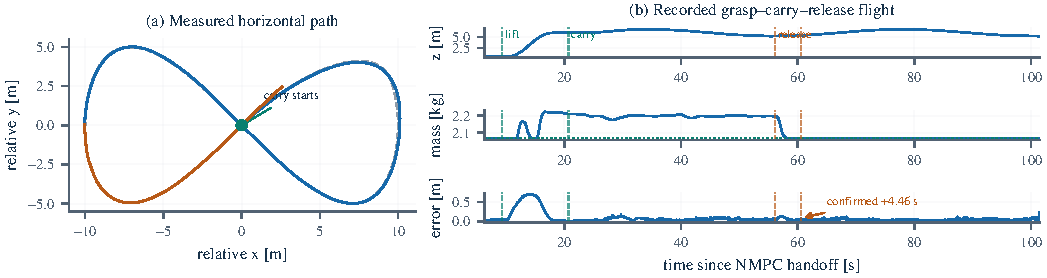
\includegraphics[width=0.95\textwidth]{figs/fig_mission.pdf}
\caption{One eventless flight from the final batch (\SI{0.15}{kg}, \SI{2}{m/s}).
Left: the measured horizontal path (blue while carrying, orange after release)
against the nominal reference including its amplitude ramp (grey dashed).
Right: recorded height, controller-consumed mass estimate, and position-error norm
through grasp, lift, carrying, release command, and confirmation.
This flight confirms in maneuver, 4.46 s after the command; it illustrates one
execution and does not replace the cohort statistics in Table~\ref{tab:complete}.}
\label{fig:mission}
\end{figure*}

The controller issues the gripper-release command itself, but deliberately does not use that
command to clear its payload model: a commanded release is not proof of physical detachment.
The proposed interface consumes only healthy, fresh $m/s/J$ frames and completes a release only
after its no-payload confidence remains above 0.90 for \SI{1.0}{s}. We report every eventless
flight in the final campaign that met the pre-registered eligibility criteria: successful MHE
payload evidence and survival to the release command. Exclusions are reported below and are not
absorbed into the completion result.

\paragraph{Paired external-event baseline}
We retain the pre-registered paired ablation rather than selecting arm~B alone after the
comparison. Arm~A is an external-event baseline: it treats the release command as the
detachment event and immediately resets payload geometry and inner-loop scaling. Arm~B is the
proposed eventless interface above. A pair enters this comparison only when both arms satisfy
the same eligibility criteria. There are 23 such pairs (8/7/8 across the three conditions); both arms complete
23/23 releases with no observed post-release instability (Table~\ref{tab:paired-event}).
Arm~A has zero confirmation delay by definition, whereas arm~B waits for physical evidence.
This comparison therefore quantifies the cost of refusing the event shortcut; it is not
evidence that arm~A detects physical detachment.

\begin{table}[tb]
\caption{Paired external-event ablation. Arm~A clears the model from the command by
construction; arm~B requires estimator evidence. The last row injects a command/physical-
detachment mismatch; ``early'' means model clearing before the DetachableJoint is removed.
The one valid but unpaired arm~B run of that row also did not clear early (0/6).}
\label{tab:paired-event}
\centering
\scriptsize
\setlength{\tabcolsep}{2.5pt}
\begin{tabular}{@{}lcccc@{}}
\toprule
condition & pairs & A compl. & B compl. & early clear A/B \\
\midrule
\SI{0.15}{kg}, \SI{4}{m/s} & 8 & 8/8 & 8/8 & -- \\
\SI{0.30}{kg}, \SI{4}{m/s} & 7 & 7/7 & 7/7 & -- \\
\SI{0.15}{kg}, \SI{2}{m/s} & 8 & 8/8 & 8/8 & -- \\
\midrule
nominal pooled & 23 & 23/23 & 23/23 & -- \\
\SI{0.15}{kg}, \SI{2}{m/s} + \SI{4}{s} hold & 5 & 5/5 & 5/5 & 5/5 / 0/5 \\
\bottomrule
\end{tabular}
\end{table}

To exercise the mismatch that motivates the paper, a fault injector received the normal
release command but retained the physical DetachableJoint for a median \SI{4.01}{s}. Twelve
arm-runs were attempted; one arm~A run never armed PX4, leaving five valid pairs and one
valid but unpaired arm~B run. In all five pairs arm~A cleared its payload model at the
command---a median \SI{4.01}{s} before physical detachment. Arm~B never cleared before
detachment in any of its six valid runs, the unpaired one included: it entered
\textsc{unresolved} in 5/6 and then confirmed a median \SI{12.45}{s} after detachment, while
the remaining run confirmed \SI{3.00}{s} after detachment without entering
\textsc{unresolved}. Within the five pairs, median position-error peaks during the
four-second hold were \SI{0.071}{m} (A) and \SI{0.068}{m} (B), so we claim a semantic safety
distinction, not a tracking advantage. All eleven valid runs had an independent Gazebo
\texttt{DETACHED} state record.

The eventless interface completed autonomous release confirmation in 31/31 eligible flights with no
observed post-release instability (Table~\ref{tab:complete}). The two-sided \SI{95}{\percent}
Clopper--Pearson interval is $[\SI{88.8}{\percent},\SI{100}{\percent}]$, so this result
demonstrates closed-loop feasibility rather than a zero failure rate.

The confirmation delay is \emph{bimodal}, and the two modes are two distinct control paths
rather than a spread within one path. In \SI{42}{\percent} of flights the no-payload
confidence crosses threshold while the vehicle is still flying the figure-eight and
confirmation completes in \SI{3.46}{s} (median; one such flight is shown in
Fig.~\ref{fig:mission}). In the remaining \SI{58}{\percent} no moment vote is available in maneuver---$\hat s$
has drifted under sustained excitation or the frozen reference never formed---so the system
reaches its \SI{12}{s} timeout, declares the payload
state \textsc{unresolved}, and executes a \SI{3}{s} smooth brake to hover; deceleration
alone restores observability and confirmation then completes at \SI{16.48}{s} (median).
Reporting one median across both paths would be misleading, so Table~\ref{tab:complete}
separates them.

In 26 of the 31 flights the payload-presence machine made exactly two transitions---one
load declaration at grasp and one empty declaration at release---with no spurious
carrying-phase transition. In the five remaining flights, all of which confirmed
in maneuver, the estimator's presence machine never declared \textsc{empty} within the logged
window (over \SI{40}{s} past confirmation); confirmation rested on the published no-payload
confidence alone, as detailed below. Four of the 31 load declarations were
raised by the estimator's own directional thrust-residual evidence rather than by sustained mass
evidence; no external grasp signal was consumed. The published first
moment decayed continuously rather than stepping to zero (Fig.~\ref{fig:moment}), confirming that recovery used the
intended estimator interface rather than the controller's release command.

\begin{table}[tb]
\caption{Eventless release completion and confirmation delay (all eligible eventless flights). Delay runs
from the release command to the frame where the no-payload confidence has held for the full
\SI{1.0}{s}, so it includes that hold. The two delay columns are distinct control paths and
must not be pooled.}
\label{tab:complete}
\centering
\scriptsize
\setlength{\tabcolsep}{3.5pt}
\begin{tabular}{@{}lcccc@{}}
\toprule
 & & & \multicolumn{2}{c}{delay median [IQR]} \\
\cmidrule(lr){4-5}
condition & $n$ & compl. & in-maneuver & via brake-to-hover \\
\midrule
\SI{0.15}{kg}, \SI{4}{m/s} & 9 & 9/9 & \SI{2.78}{s} [2.76, 2.90] & \SI{16.56}{s} [16.46, 16.60] \\
\SI{0.30}{kg}, \SI{4}{m/s} & 11 & 11/11 & \SI{7.08}{s} [6.96, 7.50] & \SI{16.40}{s} [15.76, 16.60] \\
\SI{0.15}{kg}, \SI{2}{m/s} & 11 & 11/11 & \SI{3.46}{s} [3.16, 4.36] & \SI{16.48}{s} [16.40, 16.50] \\
\midrule
pooled & 31 & 31/31 & \SI{3.46}{s} [2.86, 4.46] & \SI{16.48}{s} [16.36, 16.60] \\
\bottomrule
\end{tabular}
\\[2pt]
\footnotesize Pooled completion \SI{100}{\percent}, two-sided \SI{95}{\percent}
Clopper--Pearson CI $[\SI{88.8}{\percent}, \SI{100}{\percent}]$; overall delay max
\SI{16.70}{s}. The share of flights confirming only after the brake-to-hover maneuver is
\SI{56}{\percent}, \SI{64}{\percent} and \SI{55}{\percent} (rows in order) and
\SI{58}{\percent} pooled; the complement confirms in maneuver.
\end{table}

\paragraph{Safety boundary}
The 31/31 batch validates the interface once its release evidence is accepted; it does not
validate a universally robust detector. We therefore tested three physically distinct evidence
sources: payload quantity, directional thrust residual, and collapse of the normalized first
moment. A fast branch combining quantity and residual without moment evidence declared release
prematurely in 3/9 randomized flights during a \SI{4}{m/s} figure-eight. Loaded-flight mass
estimates could remain below the nominal empty threshold for up to \SI{48}{s}, while a dynamic
thrust excursion reached \SI{-1.69}{N}, exceeding the \SI{-1.47}{N} weight change of the
smallest payload. Neither source is therefore reliable on its own in this regime.

We rejected that branch: the estimator's unified release detector now fires only on fresh,
successful moment-collapse evidence (the slow and moment--residual paths); the legacy
mass-domain route that remains is quantified below. Ambiguous cases enter \textsc{unresolved};
a timeout does not clear the model or reset adaptive state. In a subsequent 12-flight
randomized validation, no flight declared release before the command: all 11 confirmed
releases passed through moment-gated paths (9 moment--residual, 2 slow) with a median detector
delay of \SI{1.9}{s}, and one remained safely unresolved. That validation preceded the frozen
moment reference.

\paragraph{Release paths in the final batch}
The moment-gated detector is not the only route to confirmation in the final code, and the
31-flight batch of Table~\ref{tab:complete} exercised three. The controller confirms release
when the published no-payload confidence---the product of mass, first-moment and inertia
``empty'' scores, where the moment score uses an absolute bound on $\lVert s\rVert$ rather than
the frozen-reference ratio---holds above 0.90 for \SI{1.0}{s} on healthy, fresh frames.
(i)~In 19/31 flights (9/9, 1/11 and 9/11 in the rows of Table~\ref{tab:complete}) the
moment-gated detector declared release first and the confidence followed. (ii)~In 7/31
flights, all at \SI{0.30}{kg}, the flights that reached
\textsc{unresolved}, the frozen moment reference was never established because its
low-dynamic, in-envelope sampling window never filled, so the ratio test never ran; the
confidence crossed threshold during or shortly after the brake to hover, and the estimator's
mass-domain path ($m_P<\SI{0.030}{kg}$ for 20 frames, counted only in low-dynamic flight)
declared release 0.9--\SI{3.1}{s} later. (iii)~In 5/31 flights (three at \SI{0.30}{kg}, two at \SI{2}{m/s}), all
confirmed in maneuver, the reference was likewise never established and the estimator never
declared release; confirmation rested on the confidence alone. No flight in any path declared
release before the command. The supported safety conclusion is therefore bounded: the randomized validation
supports the moment-gated detector, while the final batch shows that 12/31 confirmations did
not pass through it. Broader detector robustness remains outside the present claim.


The cohort is conditional on successful MHE payload evidence and survival to the release
command. Of 40 eventless flights, 31 were eligible: six crashed before release and three lacked
MHE payload evidence. The available logs cannot distinguish physical capture failure from
estimator non-recognition in those three cases. Confirmation delay is a median \SI{3.46}{s}
when it clears in maneuver and \SI{16.48}{s} when the vehicle must first brake to hover.

Across the paired campaign there were 81 attempts: arm~A contributed 41 attempts (30 eligible,
11 pre-release crashes), and arm~B contributed 40 (31 eligible, six pre-release crashes and
three payload-evidence failures). Only the 23 pairs in which both arms were eligible enter
Table~\ref{tab:paired-event}; all 31 eligible B flights enter Table~\ref{tab:complete}. These
are different estimands and are not substituted for one another. Tail-window tracking is not
compared: arm~B brakes to hover after an unresolved timeout, while arm~A continues the
figure-eight.
